\documentclass[11pt, a4j]{bthesis}

%-usepackage---------------------------------------%
\usepackage[dvips]{graphicx}
\usepackage{subfigure}
\usepackage{amsmath}
\usepackage{txfonts}
\usepackage{ascmac}
\usepackage{bm}
\usepackage{multirow}
\usepackage{textmf/drafts}
\usepackage{float}
\usepackage{url}
%-end usepackage-----------------------------------%

% 要旨用和文題目 英文題目
\AJtitle{マルチFPGAボードによるGoogLeNetの高速化}

% 要旨用和文題目 英文題目
\TJtitle{マルチFPGAボードによるGoogLeNetの高速化}

\Jauthor{飯塚 健介}
\Eauthor{Kensuke Iizuka}
\Kauthor{イイヅカ ケンスケ}
\StudentID{61401007}

\Boss{天野 英晴 教授}
\Tmajor{情報工学科}
\Amajor{情報工学}
\Emajor{Information and Computer Science}

%-review mode--------------------------------------%
%\pagestyle{drafts}
%\renewcommand{\baselinestretch}{1.5}
%-end review mode----------------------------------%

\begin{document}
\pagestyle{empty}

%-title--------------------------------------------%
\maketitle
%-end title----------------------------------------%


%-abstract-----------------------------------------%
\jabst{
    昨今,人工知能が最新技術のトレンドとして様々なメディアに取り上げられている.
    人工知能技術が組み込まれる自動運転,レコメンドシステム,自動翻訳などのサービスは日々の生活をより豊かにすると期待されている.
    人工知能技術を実現させる機械学習の中でも,画像認識や自然言語処理,物体検出などの分野で
    大きな貢献を果たしているニューラルネットワークは一躍注目されていて,研究開発が盛んに行われている.
    ニューラルネットワークの一種である畳み込みニューラルネットワーク(CNN: Convolutional Neural Network)は畳み込み演算を主な計算とする.
    CNNは認識精度向上を目指し様々なモデルが提案されているが
    % ここの部分をもっと充実させたい.
    年々その計算量が増加する傾向にあり,研究サイクルを早くする,データセンターでのアプリケーションとしての利用に耐えうる,
    高速化,電力性能向上が求められている.

    しかし,汎用プロセッサではその要求を満たすことができないので,各半導体メーカや研究機関は専用のアクセラレータの開発に取り組んでいる.
    日本でも国立研究開発法人新エネルギー・産業技術開発機構(NEDO)は
    「省電力AIエンジンと異種エンジン統合クラウドによる人工知能プラットフォーム」プロジェクトで
    複数のFPGA,GPU,メモリなどの異種ノードを多数接続した大規模計算基盤Flow-in-Clowd(FiC)を開発している.
    複数のFPGAは高機能スイッチノードとして多数の高速リンクが接続され,FiCの高速通信のスイッチングの役割を担う.
    このマルチFPGAシステムは主演算を行うGPUノードであるが,FPGAノードも余った計算資源を利用してAIエンジンとしての役割も担うことができる.
    本研究ではマルチFPGAシステムに2014年の国際画像認識コンペで最高精度をマークしたCNNモデルの1つであるGoogLeNetを実装し,評価した.
    % 性能でCPUの〇〇倍,GPUの〇〇倍を達成し電力効率でCPUの〇〇倍,GPUの〇〇倍を達成した.
}
\makejabstract
%-end abstract-------------------------------------%


%-contents-----------------------------------------%
\pagenumbering{roman}
\tableofcontents
\listoffigures
\listoftables
%-end contents-------------------------------------%


%-body---------------------------------------------%
\pagestyle{headings}
\pagebreak
\pagenumbering{arabic}
\setcounter{page}{1}

\chapter{序論}
{
    \label{chap:introducion}

    \section{本研究の背景}
    \label{sec:backgroud}
    人工知能と称される機械学習をベースにした技術は爆発的な普及を見せていて日夜,メディアで取り上げられるだけでなく,
    自動運転やスマートスピーカー,スマートフォン向けアプリケーションなど様々なシステムに取り込まれている.
    しかし,人工知能のさらなる普及にはその計算基盤が必要である.
    その中でも特に画像認識や物体検出などの分野で活躍する畳み込みニューラルネットワーク(CNN)はその計算の特性から
    汎用CPUでは効率よく演算処理ができない.インテルやNVDIAなど大手半導体メーカーを始めとしてGoogleやMicrsoftなども
    人工知能向け専用アクセラレータの開発に心血を注いでいる.
    各社,研究機関はGPU,ASIC,FPGAなど様々なデバイス,手法で高速化を図る.
    その中でもFPGAはその電力効率のよさ,開発周期の短さ,再構成可能であることから注目され研究がなされている.
    日本でも国立研究開発法人新エネルギー・産業技術開発機構(NEDO)は「省電力AIエンジンと異種エンジン統合クラウドによる人工知能プラットフォーム」と銘打ったプロジェクトで
    複数のFPGA,GPU,メモリなどの異種ノードを多数接続した大規模人工知能計算基盤Flow-in-Clowd(FiC)を開発している.
    このFiCはデータセンターなどに導入されるクラウドシステムである.主演算装置となる複数のGPUを複数のFPGAのスイッチノードに接続し,
    高速通信を行う.高機能スイッチノードととなるマルチFPGAは多数の高速リンクが接続され,FiCの高速通信のスイッチングの役割を担う.
    さらにこのマルチFPGAシステムはスイッチノードという役割に加え,AIエンジンとしての役割も担う.
    そこで本研究ではマルチFPGAシステムの試作ボードであるFiC-SW1を複数枚用いて,CNNのモデルであるGoogLeNetを実装し,評価を取った.

    \section{研究目的}
    \label{sec:purpose}
    本研究の目的はマルチFPGAシステム上にGoogLeNetを実装し,既存研究や汎用CPU,GPUに対して
    性能向上を目指すことである

    \section{本論文の構成}
    \label{sec:composition}
    \ref{chap:googlenet}章では実装対象であるGoogLeNetと畳込みニューラルネットワークの概要を説明する.
    \ref{chap:ficsw}章では本研究で用いるマルチFPGAシステムとそのプロジェクトの概要を紹介する.
    \ref{chap:survey}章では本研究に関連する先行研究について説明する.
    \ref{chap:parallel}章ではGoogLeNetの並列化手法について説明する.
    \ref{chap:implement}章では\ref{chap:paralell}での並列化を考慮した実装方法について説明する. 
    \ref{chap:eval}章では本研究の評価を行う. 
    \ref{chap:conclusion}では本論文の結論を述べる.
}


\chapter{GoogLeNet}
{
\label{chap:googlenet}
本研究でマルチFPGA上に実装するアプリケーションであるGoogLeNetについて説明する.
GoogleNetは畳込みニューラルネットワーク(CNN: Convolutional Neural Network)のモデルの1つである.
まずCNNの基本的な演算について説明する
\section{Convolutional Neural Network}
\label{sec:cnn}
2012年のILSVRC()で登場したAlexNetによりCNNは特に画像認識や物体検出の分野で優れた識別精度をマークしたことから世界で注目されるようになった,
CNNはその名前にも含まれているように式で表される畳み込み演算と呼ばれる行列の積和演算がその主なアルゴリズムである.
\begin{eqnarray}
	output(x, y)^{i} = input(x, y)^{i} / (k + \alpha \sum_{j=max(0, i-n/2)}^{min(N-1, i+n/2)} (a^j_{x, y})^2)^\beta
\end{eqnarray}
ニューラルネットワークは上述の畳込み演算に加えてプーリング,全結合層などの演算を動物の神経ニューロンが接続されるように層という形で積み重ねていき画像における画素値のような入力された行列が
各層を伝搬していき出力されるという構造をとっている.
これらの層において重みフィルターと呼ばれる行列で表されるパラメータと入力行列各要素について積和演算を行うため,CNNは計算量がとても多く,多量のパラメータを
利用することから多くのメモリアクセスを要する,非常にコンピュータ資源を必要とするアルゴリズムである.

\section{GoogLeNet}
\label{sec:googlenet}
GoogLeNetは2014年のILSVRCで最高精度をマークしたCNNのモデルの一つである.構成要素は上述の畳み込み演算,プーリング処理などが主であるという点においてはAlexNetなどと
違いはないが,それぞれの層の接続の仕方,層の深さが異なる,AlexNet, GoogLeNetそれぞれについて図にその全体像を示す

両者を比較すると,GoogLeNetのほうが,層がより深くなっていること,さらに横に広がっていることがわかる.
GoogLeNetは層を深くする代わりにそのフィルタサイズを小さくすることで,計算量,メモリアクセスを減らすように設計されている.
〇〇の研究によって一つの大きなフィルタによる畳込みよりも複数の小さなフィルタによる畳込みのほうがより高い精度を出すことができるとされている.
さらにGoogLeNetでは横に広がった層をInception層と名付け,これを複数層重ねる設計をしている.

\section{Inception}
\label{sec:inception}
Inception層は次の図で示される(これは図の一部を拡大したものと同じである)
これを見ると横に広がった層の中で1*1convと記されている層がある.この層ではサイズ1のフィルターを用いて,畳込み演算を行っている.
この層は,次元削減を行っている.これは入力チャネル(入力行列の深さ)に対して少ない層のフィルタを畳み込み演算することでその深さを
削減する,これによって計算量が減るだけでなく,精度向上が実現できる.
Inception層の出力の手前のDepthConcat層は横に広がった層のそれぞれの出力結果を図○のように深さ方向に結合することで
一つの行列として出力値にまとめる処理を行っている.
この特徴的なInception層を積層していくことで,GoogLeNetは構成される.表○にそれぞれの層で必要なパラメータ数をまとめる.
この表を見るとAlecNetに見られる全結合層がないことがわかる.GoogLeNetでは高い認識精度を保ったまま,計算量の多い全結合層を
削除することで全体の計算量を減らしている.
}
\chapter{FiCSW}
{
\label{chap:ficsw}
本章では,FiCシステムとマルチFPGAシステムであるFiCSWの概要を説明する.

\section{FiCの概要}
\label{sec:about_fic}
FiCはNEDOのプロジェクトとして以下のようなシステムの構成を目指している
1,様々な種類の処理装置を適材適所で組み合わせて運用する「異種エンジンシステム」とすることで,
汎用プロセッサを遥かに超える演算能力を有する
2,光通信技術の導入により,高速通信が可能なインターコネクトを実現することで
ホストプロセッサを介することなくエンジン同士を接続し通信のオーバーヘッドの小さなシステムを構築すること

人工知能計算基盤としてのクラウドシステムなので,大量データによる学習フェーズなど即時性を必要としない演算処理を担うことが想定される,
それに加え,様々なアプリケーションで柔軟にエンジンを効率よく割り当てるためにエンジン間を動的に変更することが
可能なネットワークを構成する必要がある.

\subsection{FiCのアーキテクチャ}
\label{sec:arch_fic}
FiCは3つの基板(ノード)とそれらをつなぐネットワークから構成される.ノードには本研究で用いるFPGAノードだけでなく
GPUノード,メモリノードがある.これらは図\ref{fig:arch_fic}に示すような接続により計算クラスタとして各種アプリケーションに用いられる

\begin{figure}[h]
  \centering
  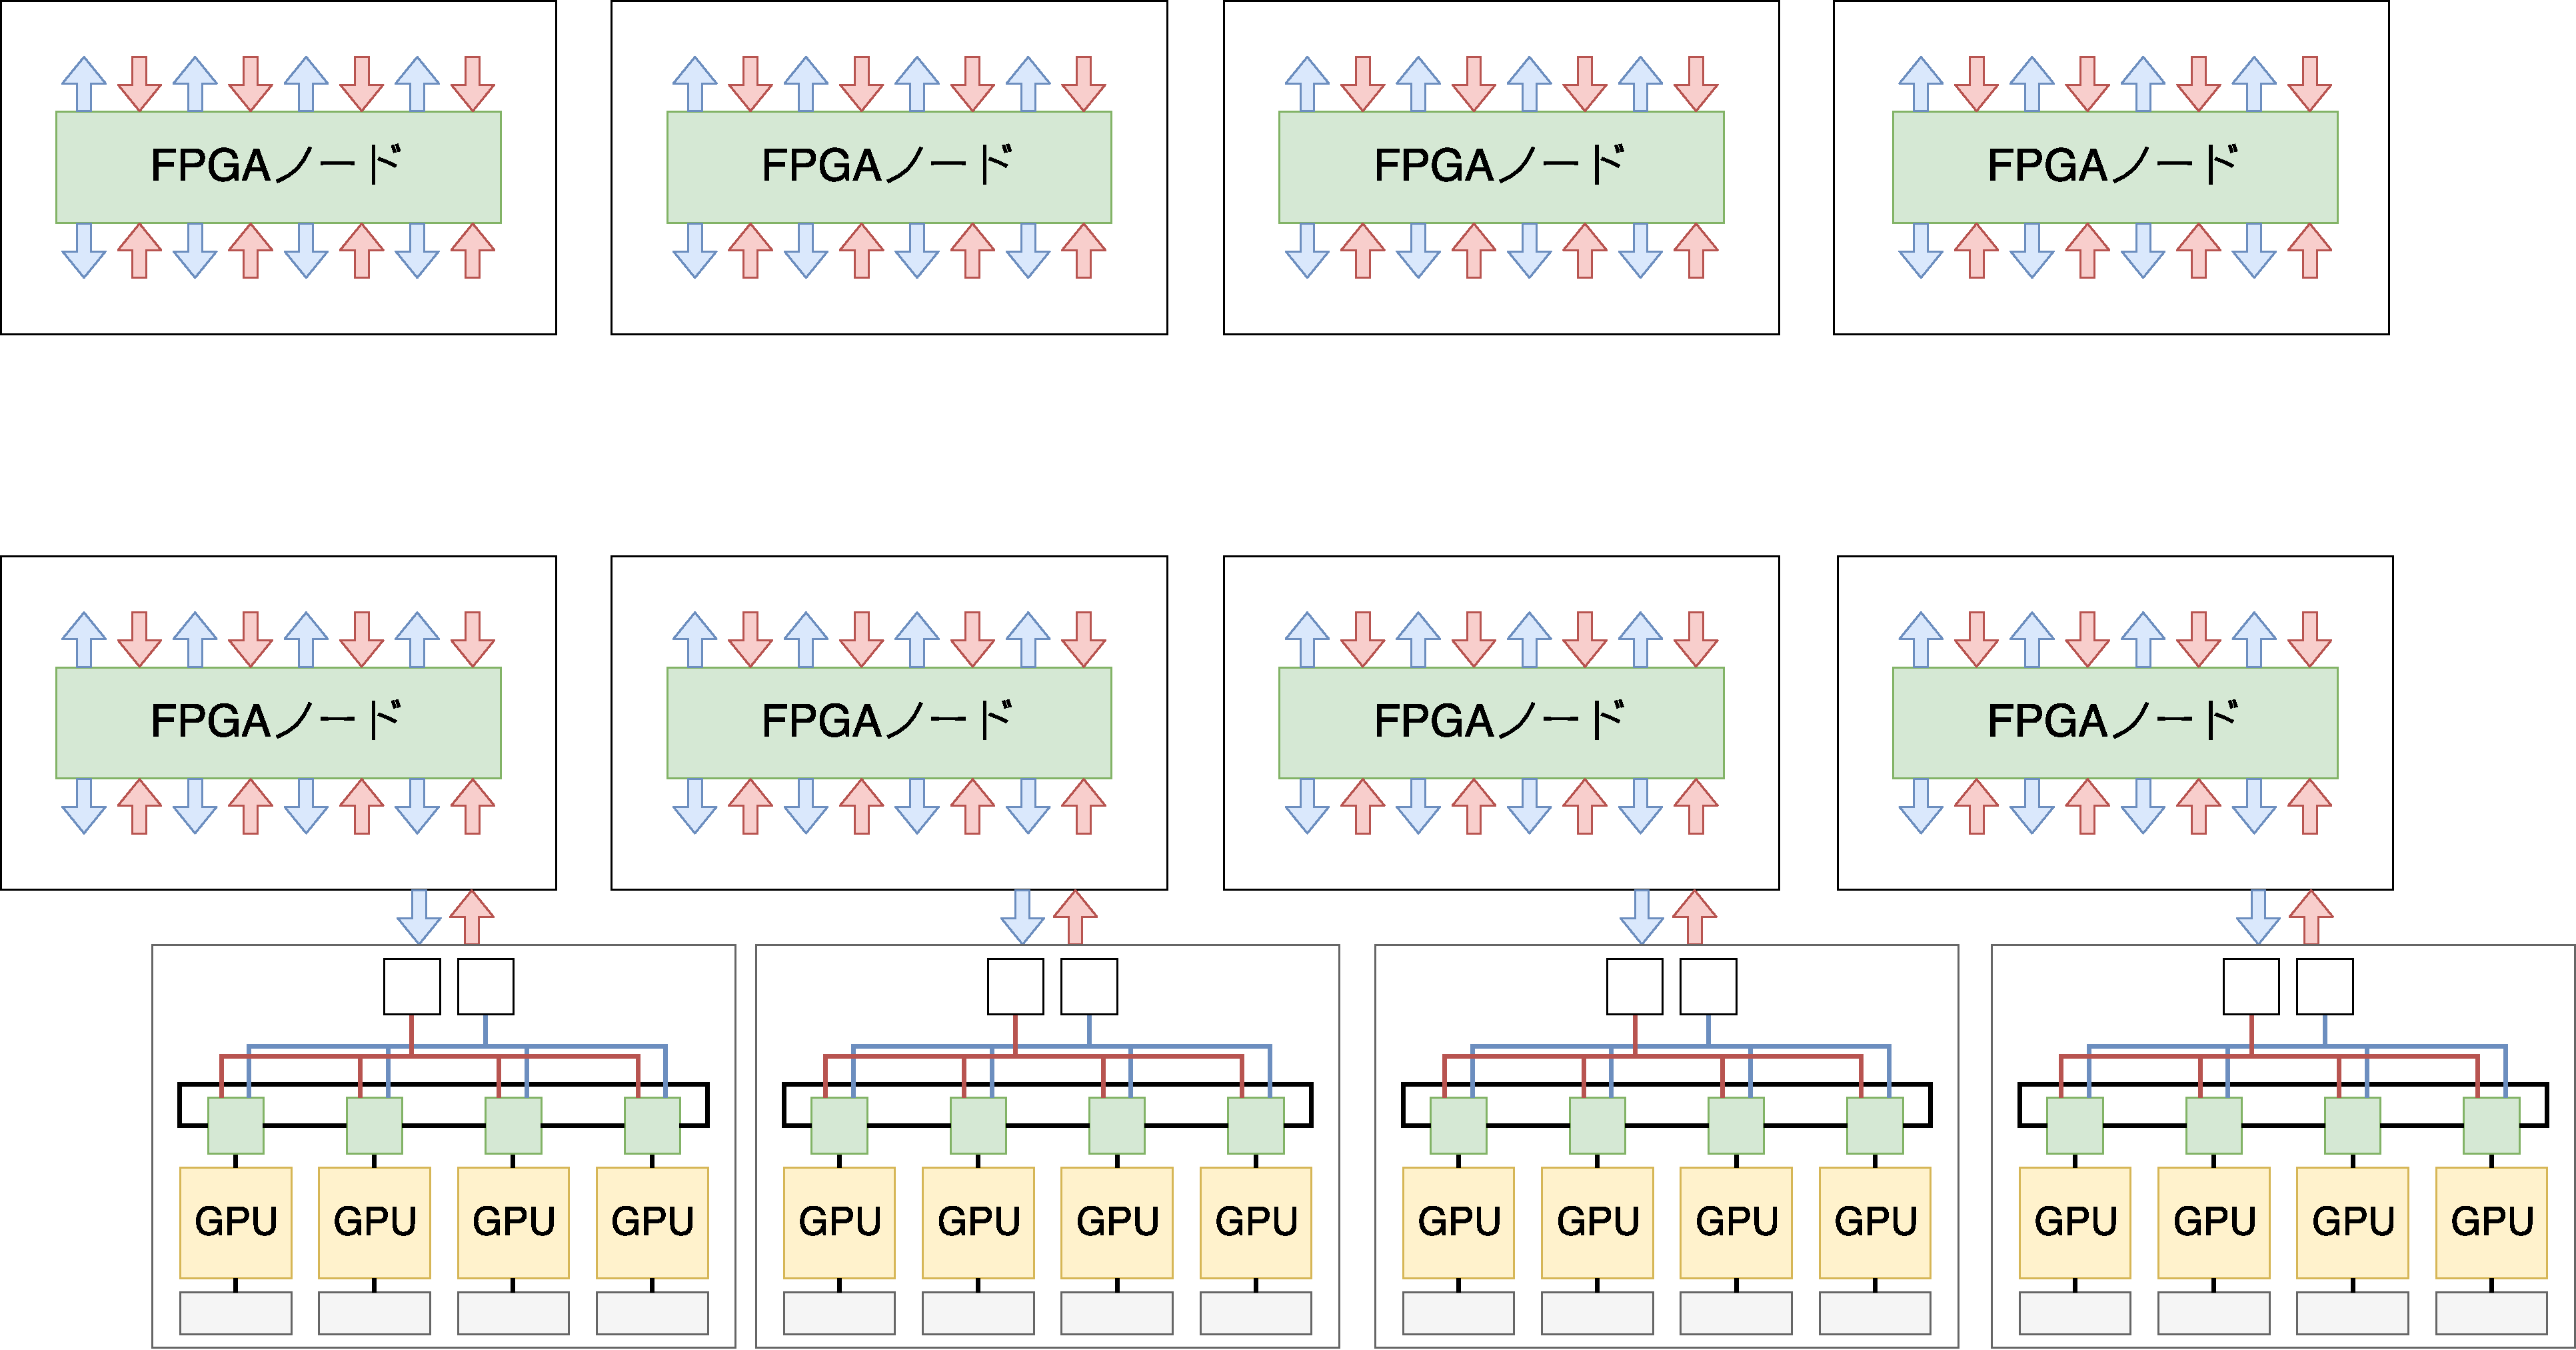
\includegraphics[width=12cm]{./chap3/fig/arch_fic.pdf}
  \caption{FiCのアーキテクチャ}
  \label{fig:arch_fic}
\end{figure}

FPGAはシステムにおいて高機能スイッチノードとしての役割が期待され。
他のFPGAやGPU,メモリノードと接続されることでGPU間の高速通信を実現するとともに
FPGAにプログラムされたデータ処理機構などを組み込むことでホストプロセッサの介在を不要とする.
メモリノードはFPGAノードに接続されることで,個々のGPUに大容量DRAMをもたせる必要がなくなり,GPUデバイスへのメモリコピーを
なくすことができ,メモリの利用効率を向上させることができる.

\section{FiC-SWの概要}
\label{sec:about_ficsw}
FiCにおいて高機能スイッチとなるFPGAボードはFiCSWと名付けられ,その試作ボードは図\ref{fig:ficsw}である.

\begin{figure}[h]
  \centering
  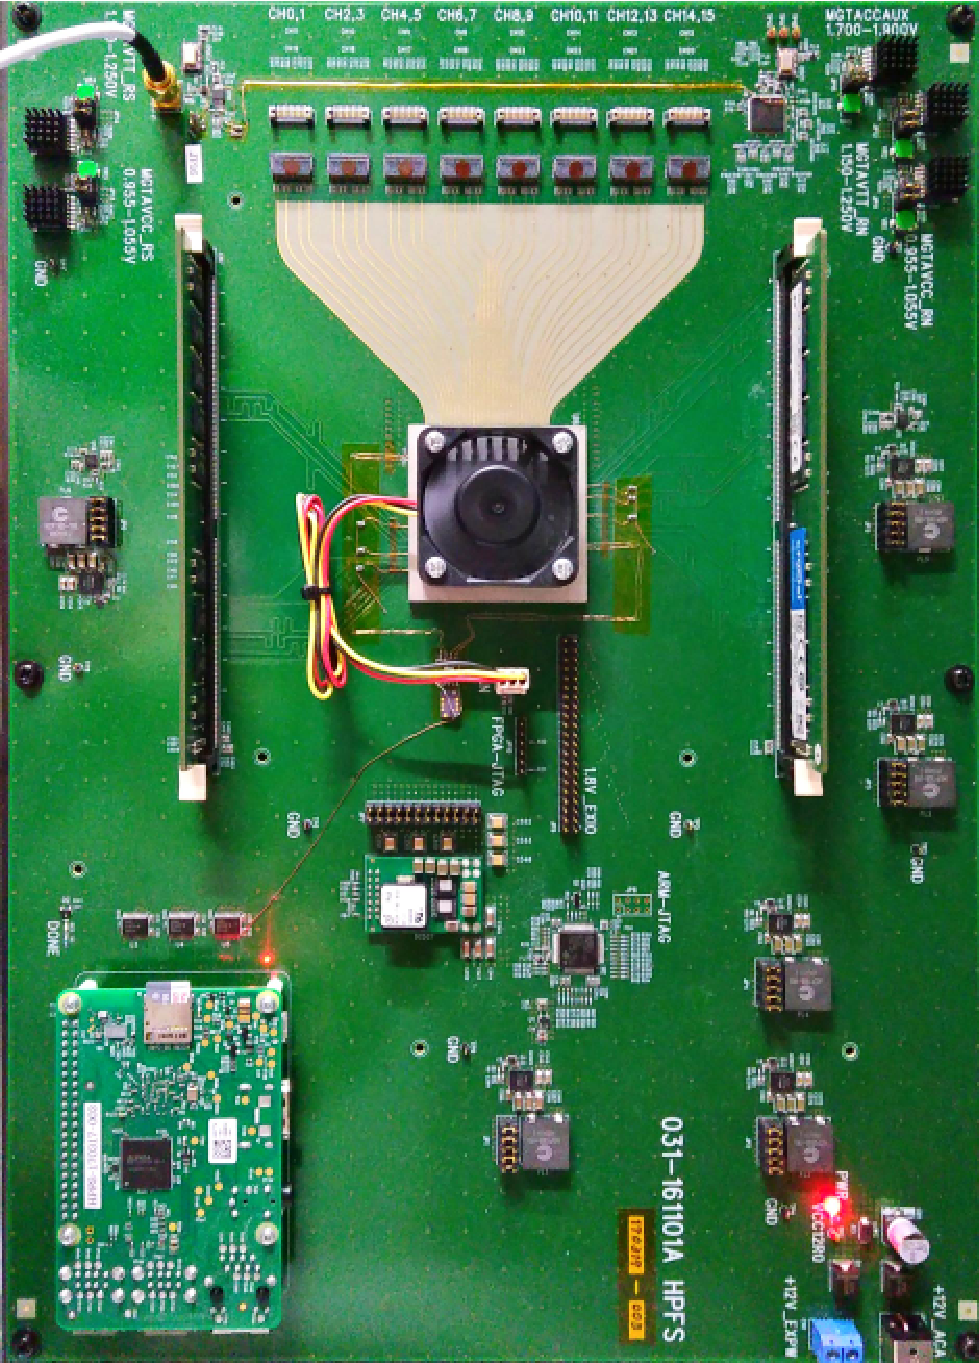
\includegraphics[width=12cm]{./chap3/fig/ficsw.pdf}
  \caption{FiC-SWの試作ボード}
  \label{fig:ficsw}
\end{figure}

図\ref{fig:ficsw}中に赤枠で囲まれた4つの要素で構成されている。
図の注釈の順に
1,Xilinx社製のUltraScale XCKU095-FFVB2104
2,高速シリアルリンク8チャネル,32リンク
3,16GBのDRAM2バンク
4,Raspberry Pie3
を搭載している。
Raspberry Pie3を用いることで,FPGAを遠隔操作して動的に再構成することができる.

\section{FiC-SWでの通信様式}
\label{sec:ficsw_communication}
FiCでは将来的に広帯域光通信技術をシステムの相互接続ネットワークに用いることが想定されている.
光信号のままスイッチすることで数十Tbpsの性能をもつインターコネクトをコストを抑えながらクラウド内で利用する
ことができる.
光信号はサーキットスイッチを用いることが現実的である.
今回のボードは従来の電気信号による通信を行うが来たる光通信の将来を想定して,サーキットスイッチによるネットワークを構成する.
サーキット数を増やすために時分割多重(TDM: Time Division Mutipling)による通信様式をとる.

図\ref{fig:arch-sw}は4リンクからなるシリアル入力から同じく4リンクからなるシリアル出力へのスイッチの模式図である。
各リンクが4スロットを有していると仮定している。図中に示される入力スロットと出力スロットの接続が回線を確立する。
図の破線矢印で示されるように1スロットから複数スロットへの出力を設定することも可能なので、
容易にブロードキャストを行える。

 \begin{figure}[h]
   \centering
   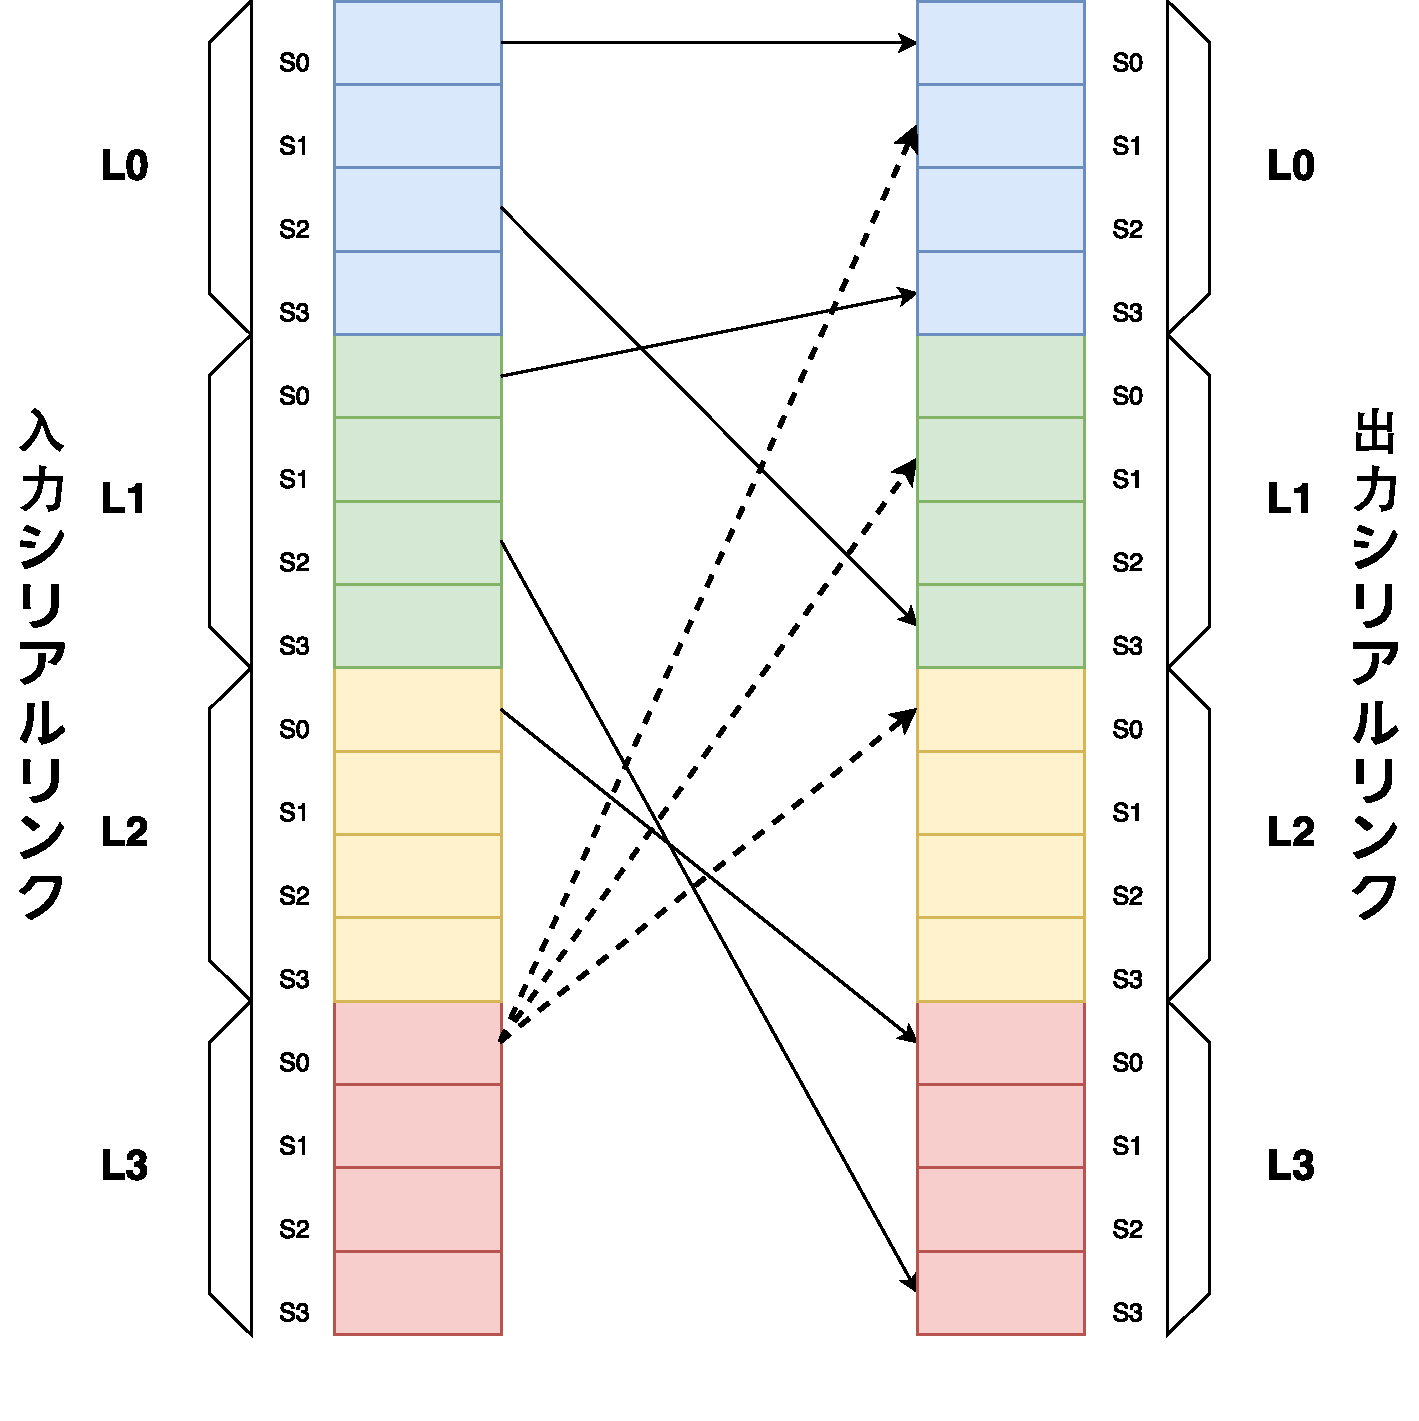
\includegraphics[width=12cm]{./chap3/fig/arch_sw.pdf}
   \caption{FiCのアーキテクチャ}
   \label{fig:arch-sw}
 \end{figure}

}

\chapter{関連研究}
{
\label{chap:survey}
}
\chapter{GoogLeNetの並列化検討}
{
\label{chap:parallel}

\section{概要}
本章ではまず,GoogLeNetの並列化検討を行う要素を明確にする.
次に並列化検討要素ごとに考察を行う.
本研究では次の3つについて並列化を検討する.
\begin{itemize}
   \item Inception層 
   \item 畳み込み演算 
   \item Pooling処理 
\end{itemize}
\section{Inception層の並列化}
\label{sec:inception_para}
表\ref{table:googlenet}からもわかるようにGoogLeNetはサイズの違いはあるが,Inception層がその大半を占めている.
これがInception層に注目した理由である.
Inception層は図\ref{fig:para_inception}に示すように4つの計算に分割することができる.
\begin{figure}[h]
  \centering
  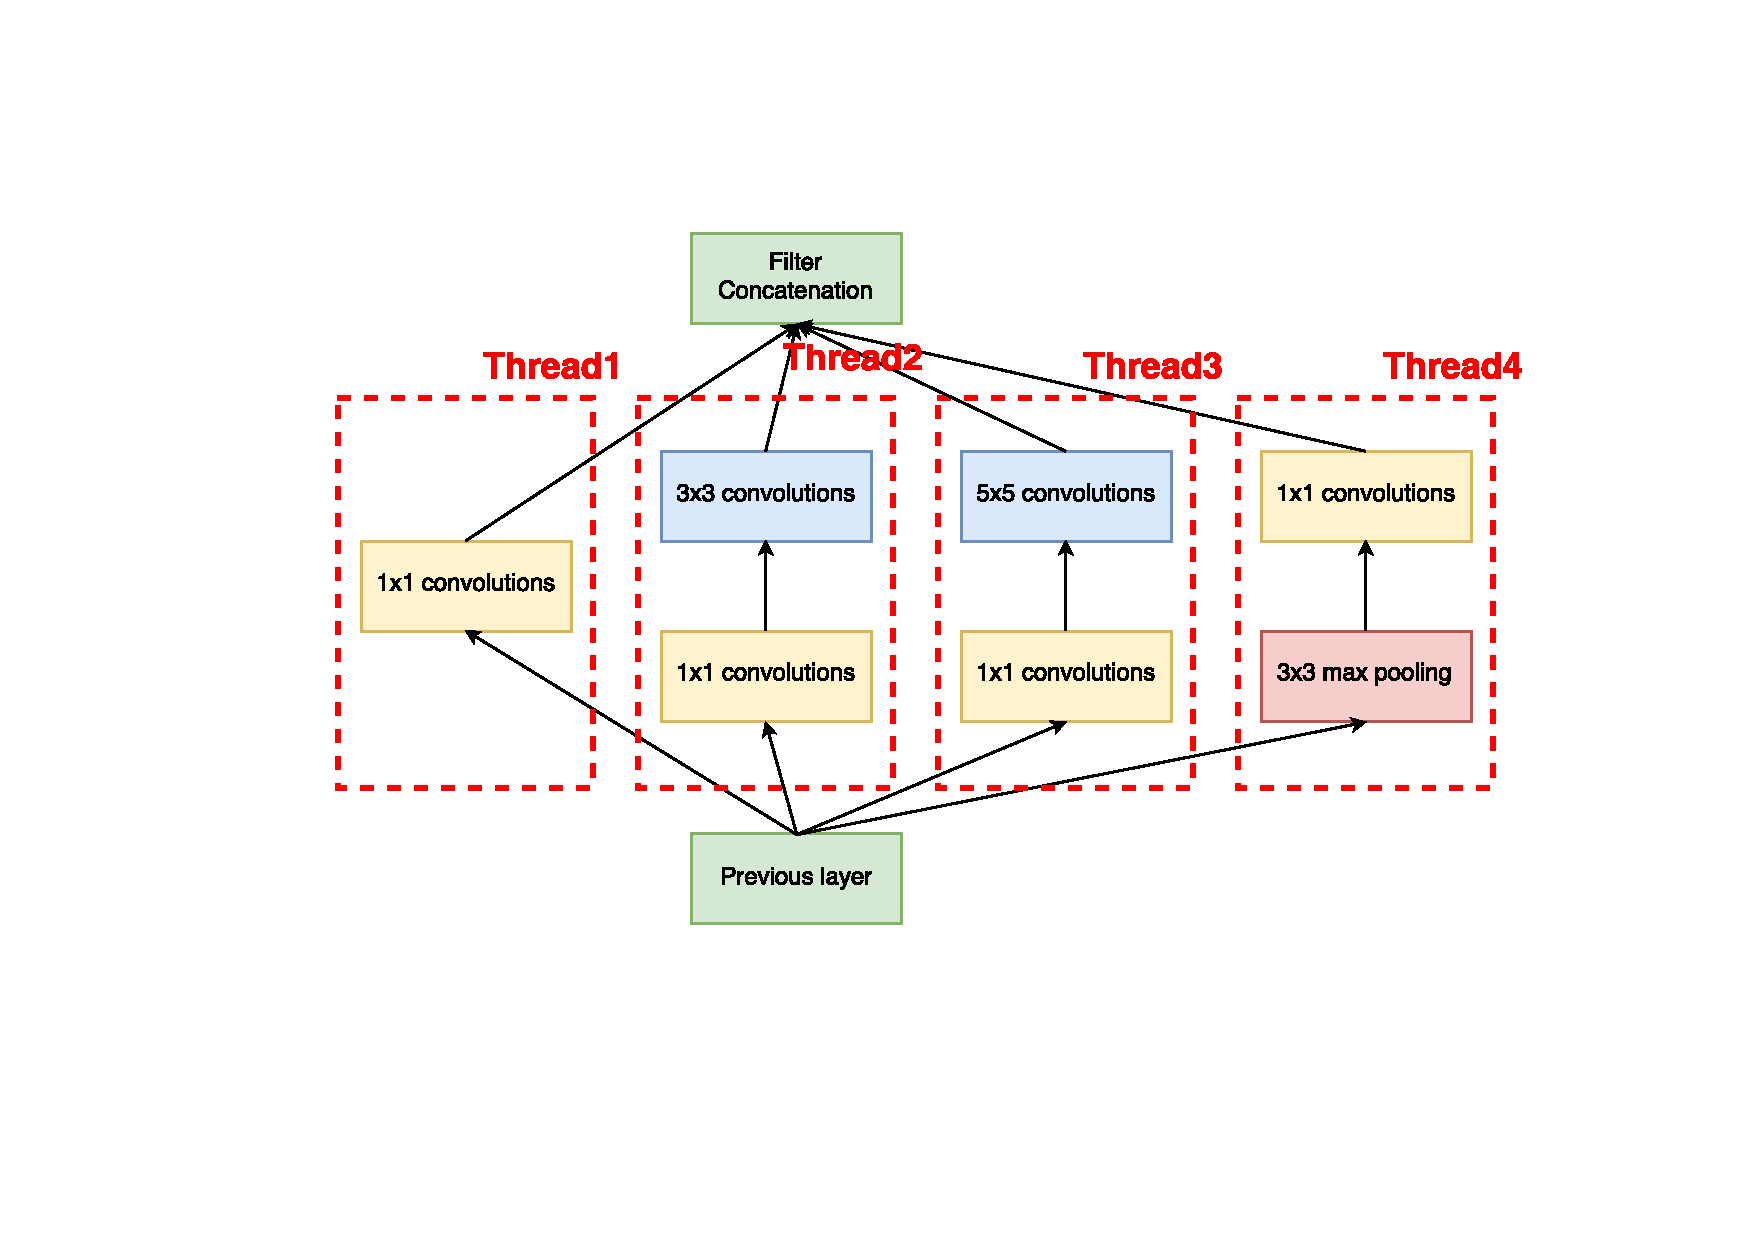
\includegraphics[width=12cm]{./chap5/fig/para_inception.pdf}
  \caption{Inception層の並列化}
  \label{fig:para_inception}
\end{figure}
便宜上図に示すようにThread1からThread4と名付けて議論する.
各スレッドには前層の出力特徴マップがそれぞれ入力特徴マップとしてブロードキャストされる.
% 各スレッドは最後にそれぞれの出力特徴マップを図\ref{fig:depth_concat}に示すように深さ方向に結合するまでの間は互いに依存せずに
% 演算を行うことができる.
% \begin{figure}[h]
%   \centering
%   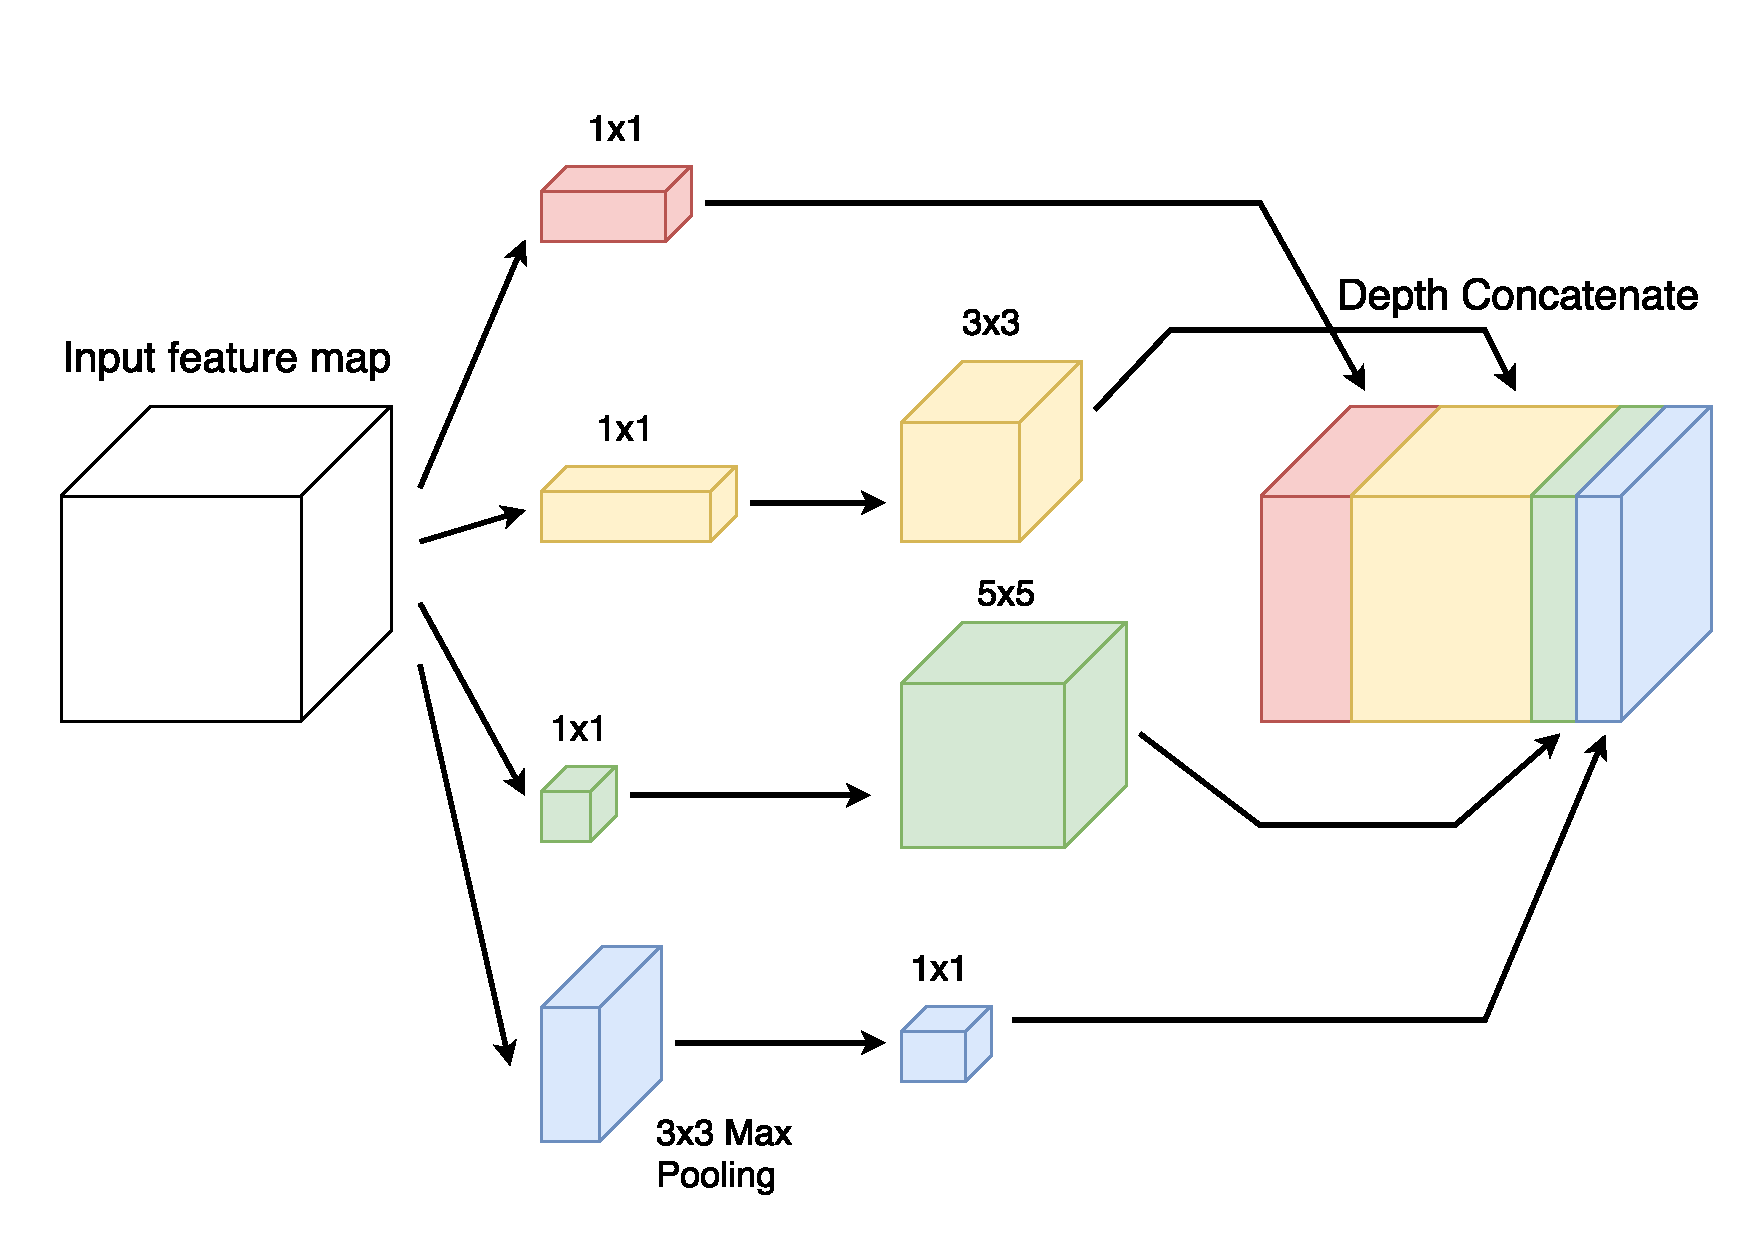
\includegraphics[width=12cm]{./chap5/fig/depthconcat.pdf}
%   \caption{}
%   \label{fig:depthconcat}
% \end{figure}
このことからInception層全体の並列化を考えると各スレッドごとに並列化することができる.
マルチFPGAに搭載する際には各スレッドごとに1枚のボードを割り当てるだけでなく,計算処理の重たいスレッドに関しては,
スレッド内の畳込み演算部などを並列に処理することができるので,あるスレッド内の処理も複数FPGAボードに割り当てることが可能である.

\section{畳み込み演算の並列化}
\label{sec:conv_para}
畳み込み演算の並列化を検討する.
CNNはその名の通り畳み込み演算が主演算となるのでこの並列化については\ref{chap:survey}で挙げた関連研究をはじめ,様々な研究で検討される.
畳み込み演算はその演算の性質上,とくにデータ並列度が高い.
本研究では重みフィルタパラメータを各FPGAボードのオンチップメモリ(BRAM)に保存し,外部からの入力特徴マップとの演算を行い,出力特徴マップを
求めるという設計を行う.これはあるFPGAがネットワークの特定の層のある箇所のみの演算を行い次々とFPGAボードを伝搬させていくという設計方針を満たす
ためである.次々と入力値をFPGAが受け取りストリーム処理を行うことを想定している.
畳み込み演算の並列化には次のようなものが考えられる.
\begin{itemize}
    \item 出力値分割
    \item 入力値分割
\end{itemize}
それぞれについて以下で詳しく述べる.
\subsection{出力値分割}
\label{subsec:para_output}
出力特徴マップを分割することを考える.出力特徴マップ同士には依存性がないが,次層での入力値となることを考えると,
すべての特徴出力マップが揃うのを待つ必要がある.
この並列化の様子を図\ref{fig:conv_para_output}に示す.
\begin{figure}[h]
    \centering
    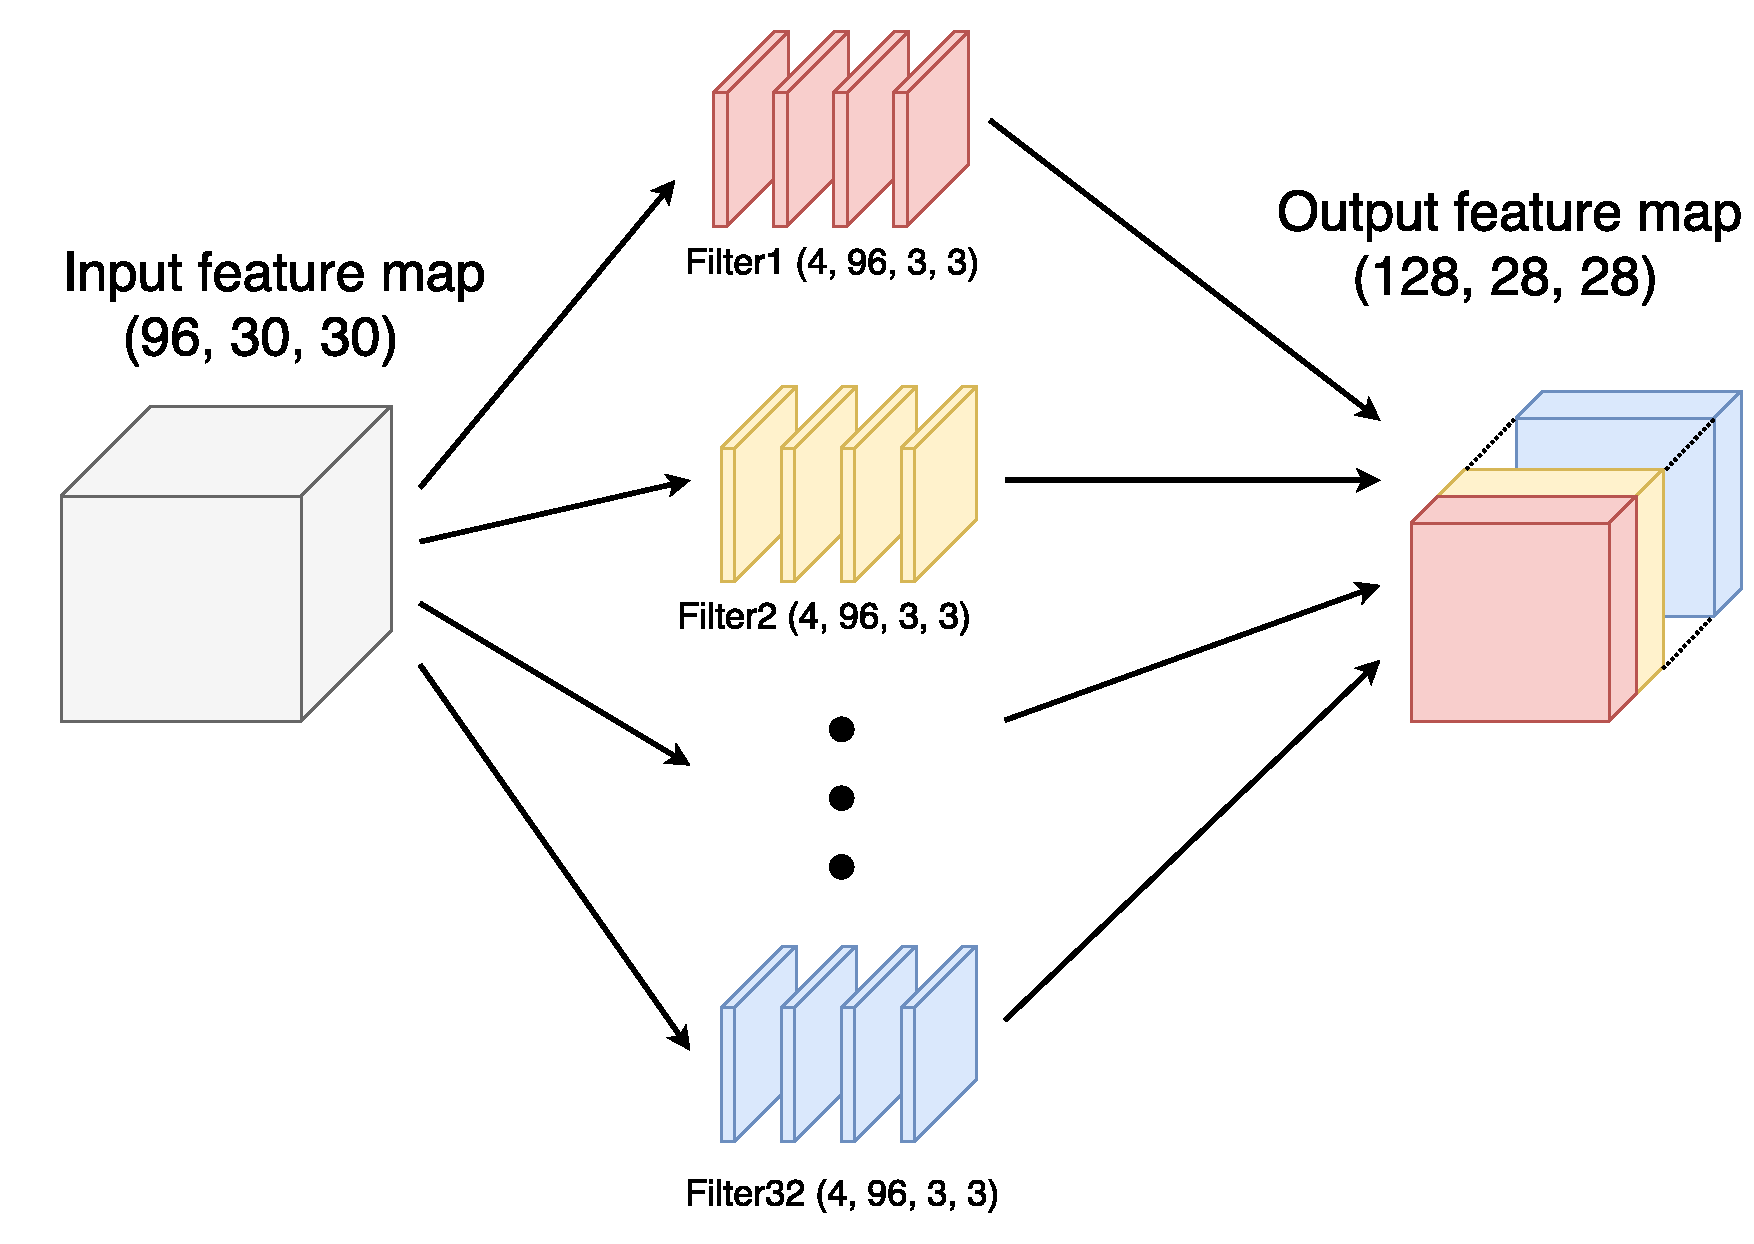
\includegraphics[width=12cm]{./chap5/fig/conv_para_output.pdf}
    \caption{出力値分割}
    \label{fig:conv_para_output}
\end{figure}
図中ではInception3a層のThread2の3$\times$3畳み込み演算の入出力サイズを用いている.
入力サイズ(96,30,30) に対して重みフィルタサイズ(128,96,3,3)の重みとの演算を行い,出力サイズ(128,28,28)に対して,32並列化を実行している.
並列化された各ノードは入力サイズ(96,30,30)を受け取り出力サイズ(4,28,28)を出力する.
こうすることで逐次的に処理するときと比較して理論的には32倍の速度性能を達成することができる.
しかし演算の最後に並列演算したそれぞれの出力特徴マップをDepthConcat層の処理のように深さ方向での結合をしなければならない.
\subsection{入力値分割}
\label{subsec:para_input}
入力値について並列化することも考えられる.入力特徴マップのサイズが大きいものについて
分割して処理することでスループットの向上の可能性がある.
この並列化の様子を図\ref{fig:conv_para_input}に示す.
\begin{figure}[h]
    \centering
    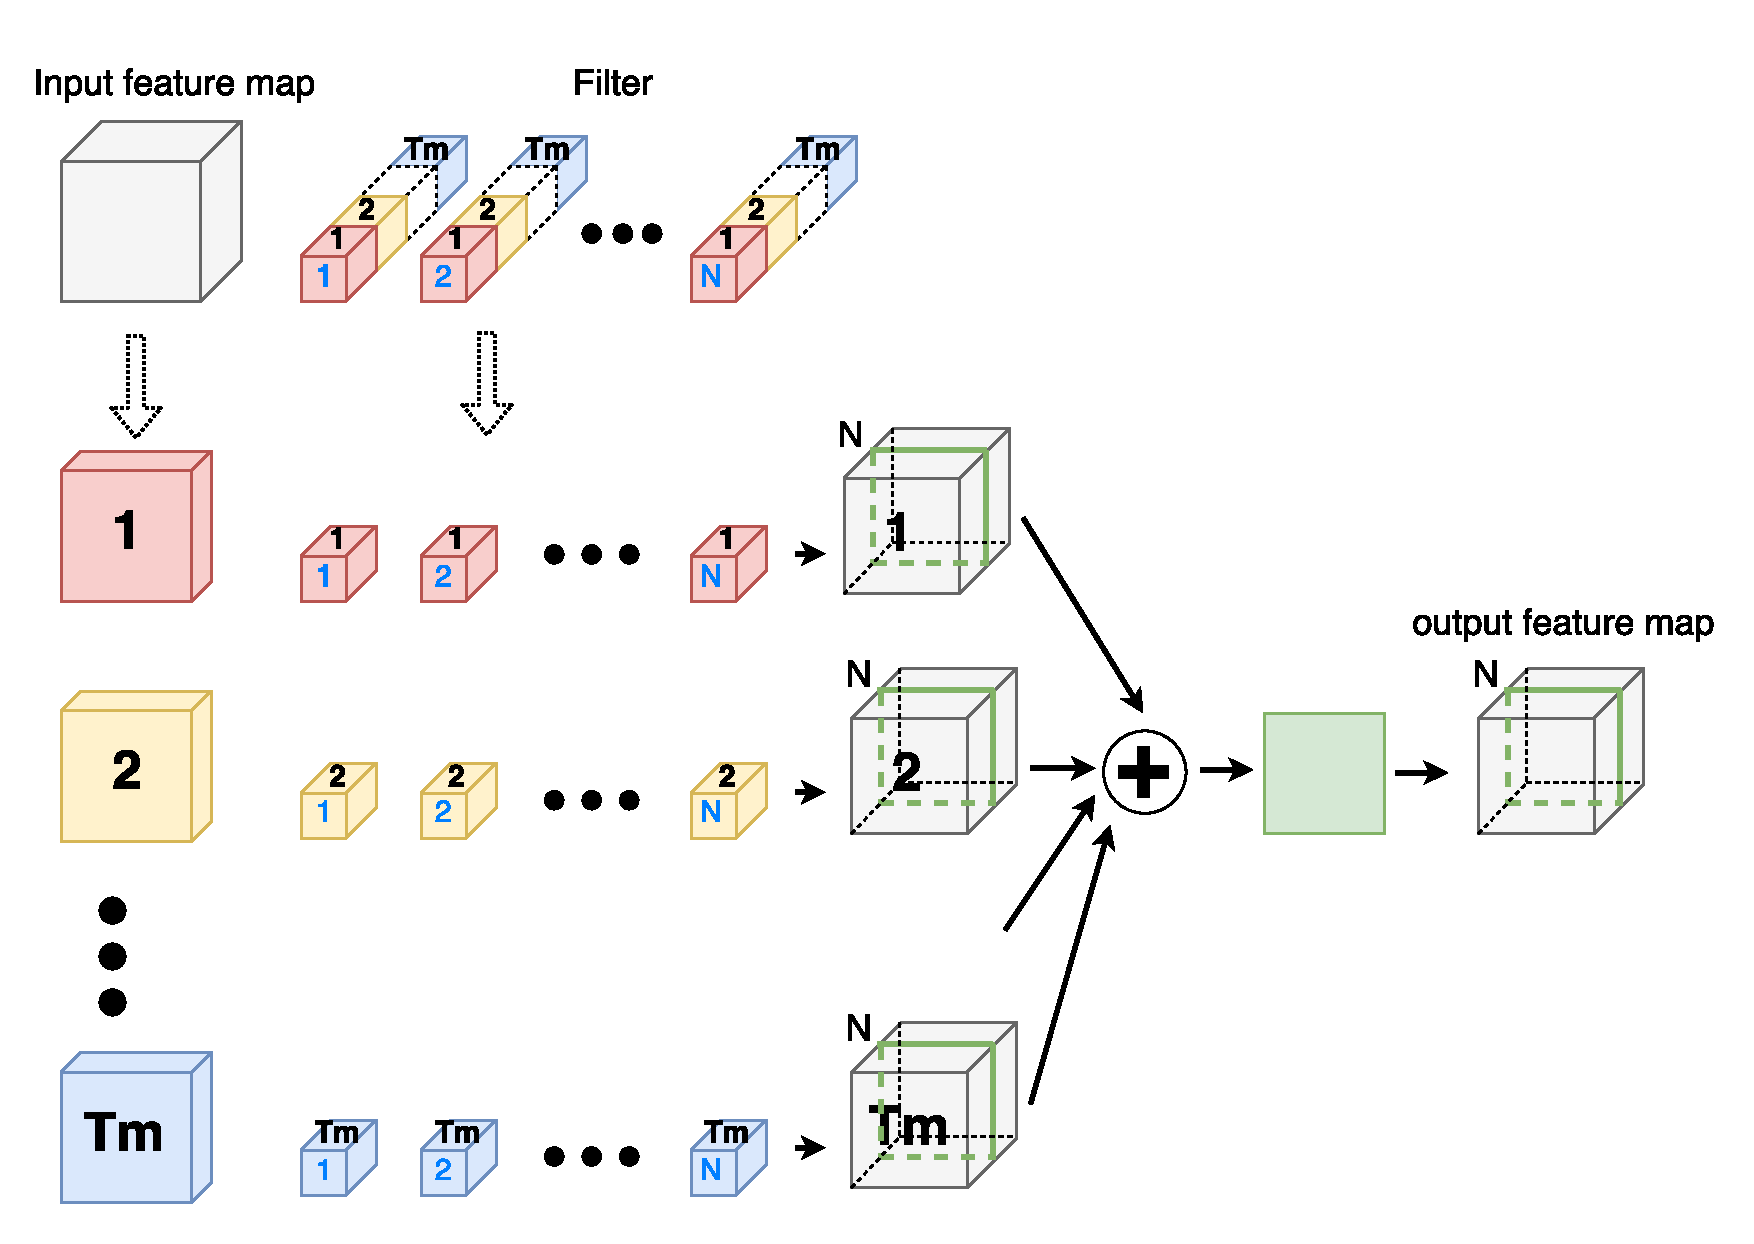
\includegraphics[width=12cm]{./chap5/fig/conv_para_input.pdf}
    \caption{入力値分割}
    \label{fig:conv_para_input}
\end{figure}
ここでも同じくInception3a層のThread2の3$\times$3畳み込み演算の入出力サイズを用いて説明する.
16個に入力特徴マップを分割するとそれぞれ(6,30,30)の入力サイズとなる.これに対し128個の(96,3,3)のサイズも16個に分割し(6,3,3)のサイズにする.
分割された入力特徴マップは対応する128個の分割された重みフィルタと畳込み演算を行い(128,28,28)の中間特徴マップを得る.
この16個の中間特徴マップのそれぞれの深さd $(1 \leq d \leq 128)$の二次元特徴マップの総和をとることで最終的な出力特徴マップの深さdの二次元特徴マップが得られる.
この操作を各dに対して行うことで最終的な出力特徴マップを得ることができる.
分割された入力特徴マップと重みフィルタはそれぞれ並列に演算が可能である.

}
\chapter{実装}
{
\label{chap:implement}
本章では\ref{chap:parallel}章の並列化に対する検討を元にして、FPGAに実装するアクセラレータについて解説する。
\section{スレッド並列化の実装}
\label{sec:thread_impl}
図\ref{fig:para_inception}で示した4つの計算スレッドについて、各スレッドにそれぞれ1枚のFPGAで演算を行うようにする。

\section{スレッド内モジュールの実装}
\label{sec:module_impl}
FiCのマルチFPGAシステムでは、流れてきたデータをそれぞれのFPGAボードでの処理を終えて、次のFPGAに出力を渡す、というフローが想定される。
そのため各ボードでは特定の演算処理のみを実行すればよいので\cite{optimized}のように複数のサイズの畳み込みを行うことは考えずに、
それぞれの層に適した入出力サイズのモジュールを実装することが可能である。また特定の層の重みフィルタのみをBRAMに保存して読み出し演算を行う。
各スレッドのモジュールはまず、ブロードキャストされる同一サイズの入力値を受け取る。その後、BRAMの重みフィルタとの畳み込み演算を行う。
図\ref{fig:thread_module}にモジュールの模式図を示す。
\begin{figure}[h]
    \centering
    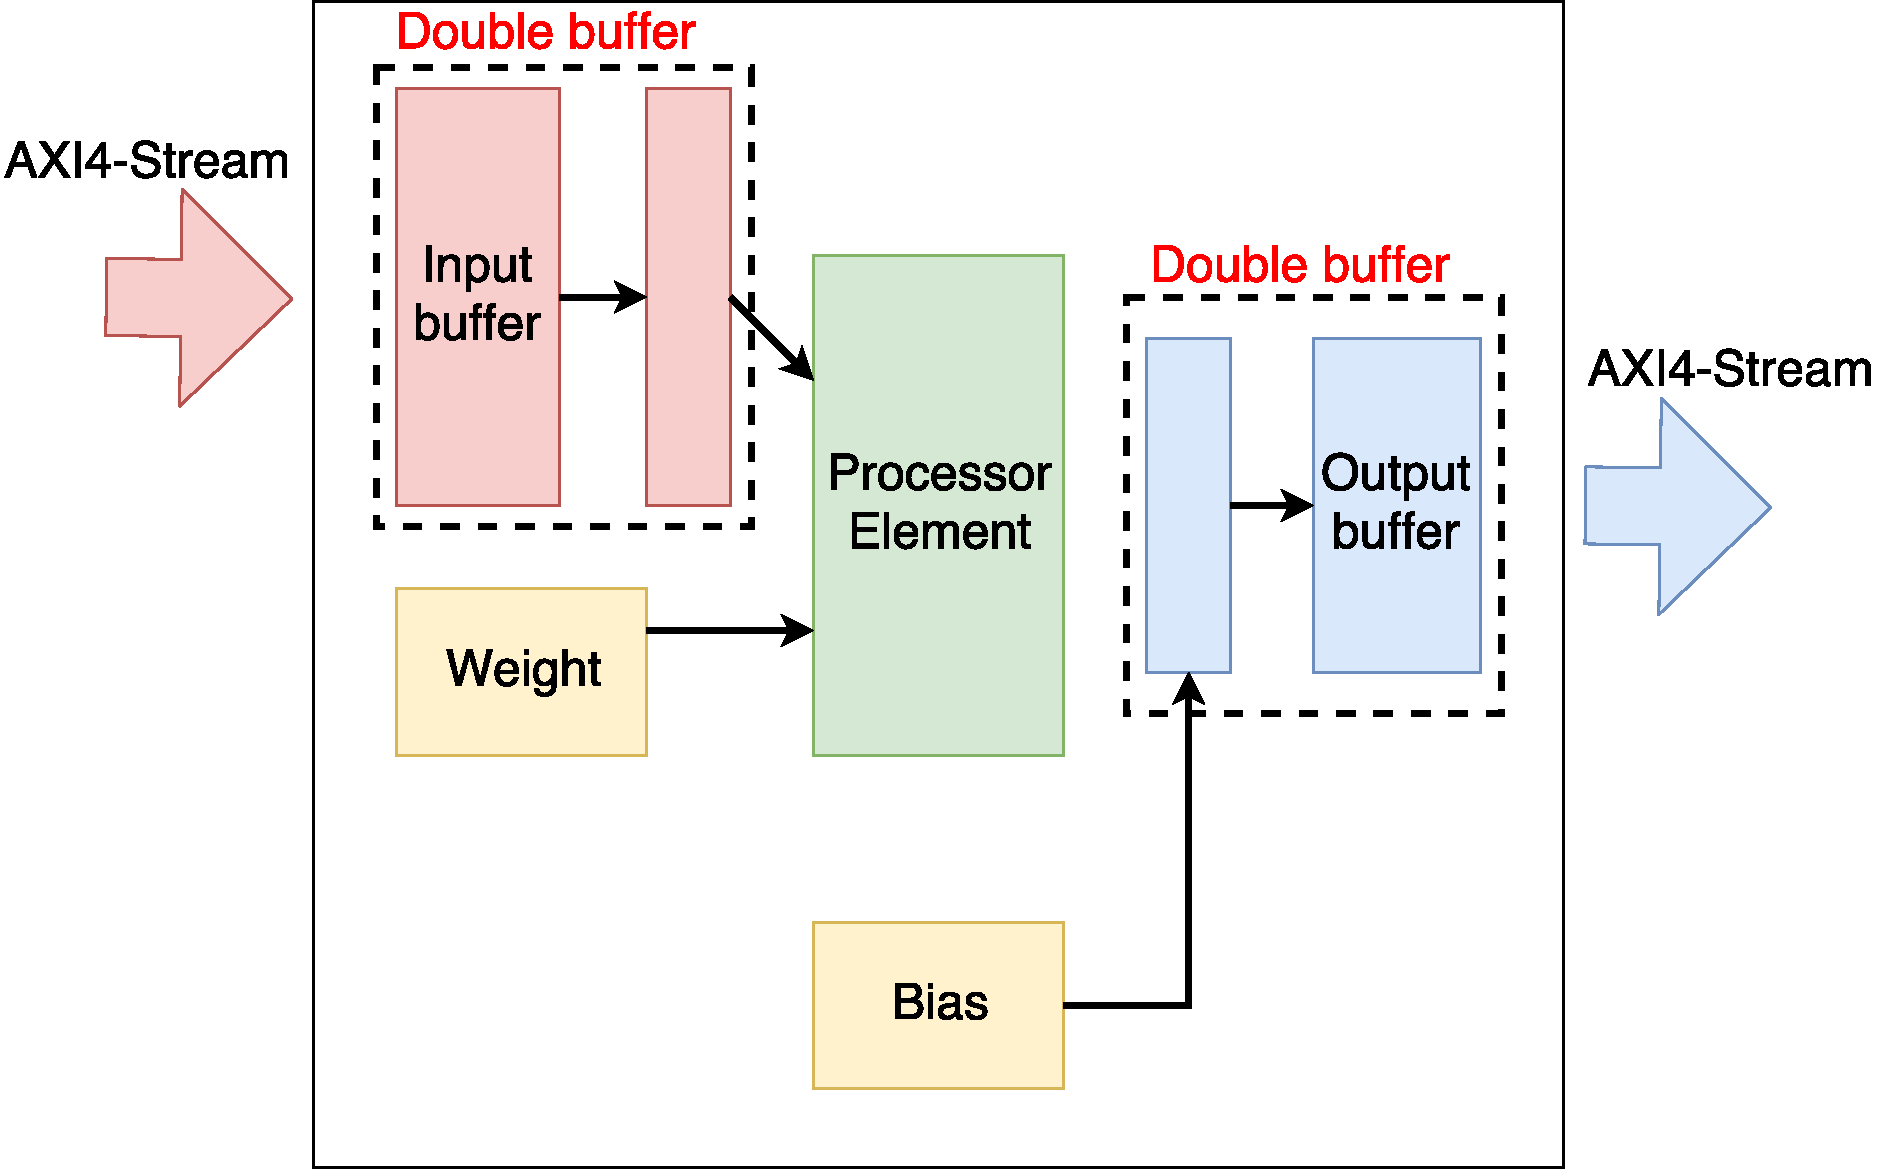
\includegraphics[width=12cm]{./chap6/fig/thread_module.pdf}
    \caption{モジュールの模式図}
    \label{fig:thread_module}
\end{figure}
入出力のインターフェイスにはXilinxが提供するAXI4-Streamを利用する。
AXI4-Streamはデータストリーム用のインターフェイスである。これにより入出力データをストリーム形式で送受信できる。
図\ref{fig:thread_module}に示すように入出力、重みフィルタにダブルバッファを設けることで演算に必要なデータを受け取ったら、
演算を行うと同時にもう片方のバッファで次のデータの書き込みが可能となる。

畳み込み演算はPEで行う。図\ref{fig:para_inception}で示した4つの計算スレッドのうちThread2、Thread3、Thread4については畳み込みやpooling処理
が連続して行われているので図\ref{fig:thread_module}が2つ接続するようなモジュールとなる。ストリーム処理を行い、パイプライン化するためにモジュール間には
バッファを設ける。

\section{畳み込み演算器の実装}
\label{sec:conv_impl}
\ref{sec:module_impl}節で述べたモジュールの模式図内のPE部の設計は\cite{optimized}を参考にした。
ここでは\ref{code:conv}に示す、畳み込み演算のCコードをループタイリングによって分割することで並列化することを考える。

\begin{itembox}[1]{畳み込み演算のCコード}
    \label{code:conv}
    \begin{verbatim}
    for (int r = 0; r < R; r++)
      for (int c = 0; c < C; c++)
        for (int to = 0; to < M; to++)
          for (int ti = 0; ti < N; ti++)
            for (int i = 0; i < K; i++)
              for (int j = 0; j < K; j++)
                output[to][r][c] +=
                  input[ti][S*r+i][S*c+j] *
                  weight[to][ti][i][j];
    \end{verbatim}
\end{itembox}

\begin{itembox}[1]{出力特徴マップチャンネルで並列化された畳み込み演算のCコード}
    \label{code:conv_tile}
    \begin{verbatim}
    for (int r = 0; r < R; r++)
      for (int c = 0; c < C; c++)
        for (int to = 0; to < M; to += Tm) //Tmごとに出力を分割
          for (int ti = 0; ti < N; ti++)
            for (int i = 0; i < K; i++)
              for (int j = 0; j < K; j++)
                output[to][r][c] +=
                  input[ti][S*r+i][S*c+j] *
                  weight[to][ti][i][j];
    \end{verbatim}
\end{itembox}

\ref{code:conv_tile}がループタイリングを行った疑似コードである。$T_m$が\ref{sec:conv_para}節で説明した、出力値による分割である.
この疑似コードに倣って演算モジュールを作ると図\ref{fig:conv_pe}のような演算器を設計できる。

\begin{figure}[h]
    \centering
    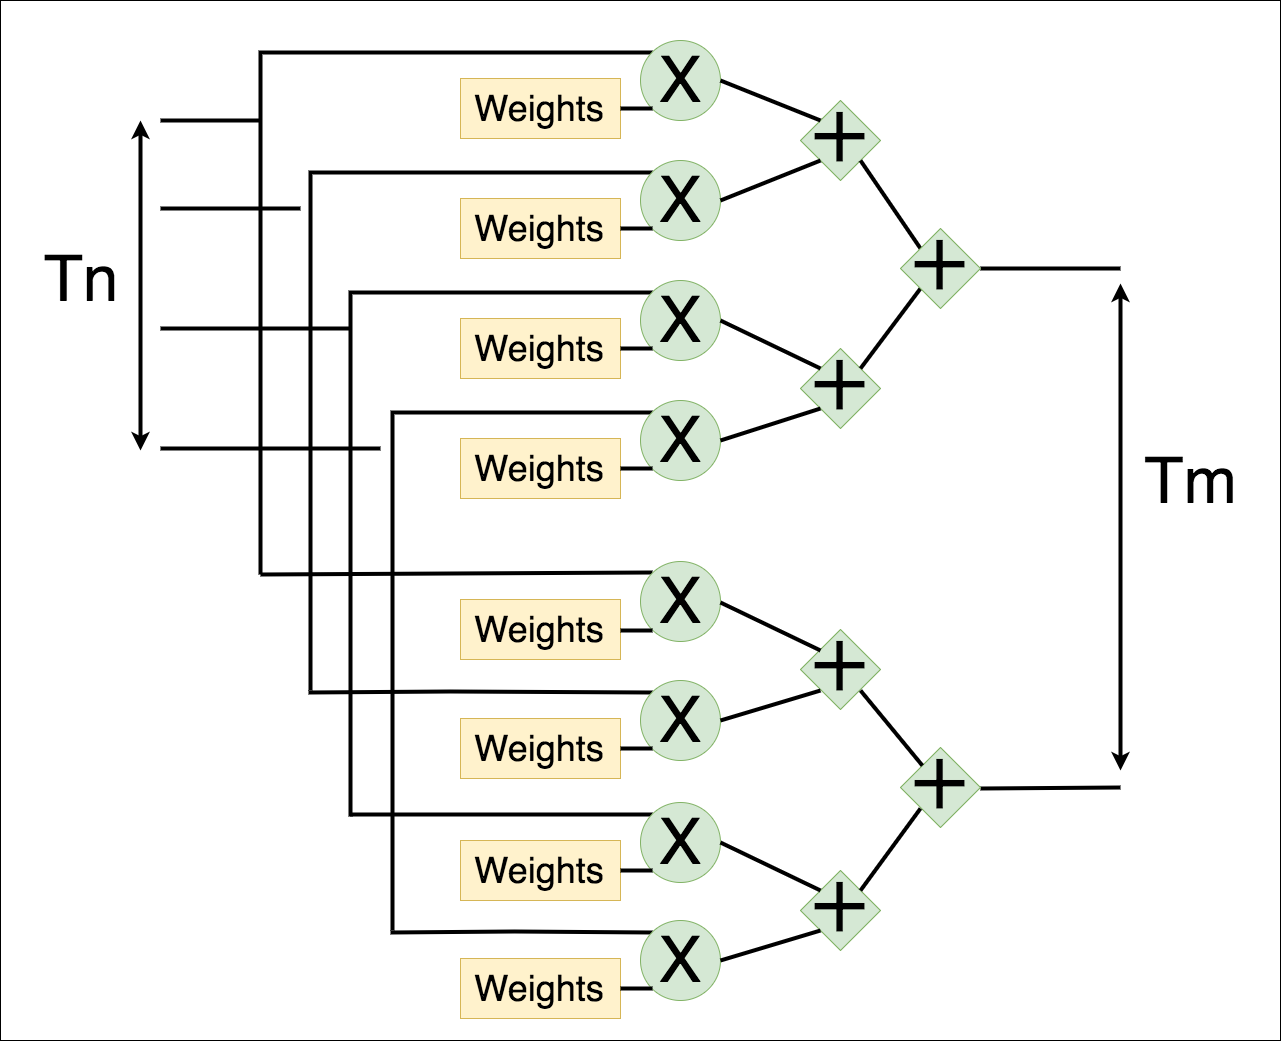
\includegraphics[width=12cm]{./chap6/fig/ucla_pe.png}
    \caption{畳み込み演算器の模式図}
    \label{fig:conv_pe}
\end{figure}

この演算器は複数の積和演算器を並列に並べたものとなっている.この演算器は$T_n$個の入力値と$T_n \times T_m$個の重みから
$T_m$個の出力値を得る.
\section{maxpooling演算器の実装}
\label{sec:max_impl}
maxpooling処理は式\ref{eq:pool}で示された最大値を取る演算を行う。
カーネルサイズの領域を入力特徴マップから抽出し、その領域内での最大値を取得し出力特徴マップに書き込むという処理を行う。
領域内の各要素について逐次的に前後の値を比較し、出力値の候補を探していく処理となるが、本研究では高速化を図るため、トーナメント方式に
値を比較する演算器を実装した。その模式図をmaxpooling処理の具体例とともに図\ref{fig:maxpool_pe}にモジュールの模式図を示す。
\begin{figure}[h]
  \centering
  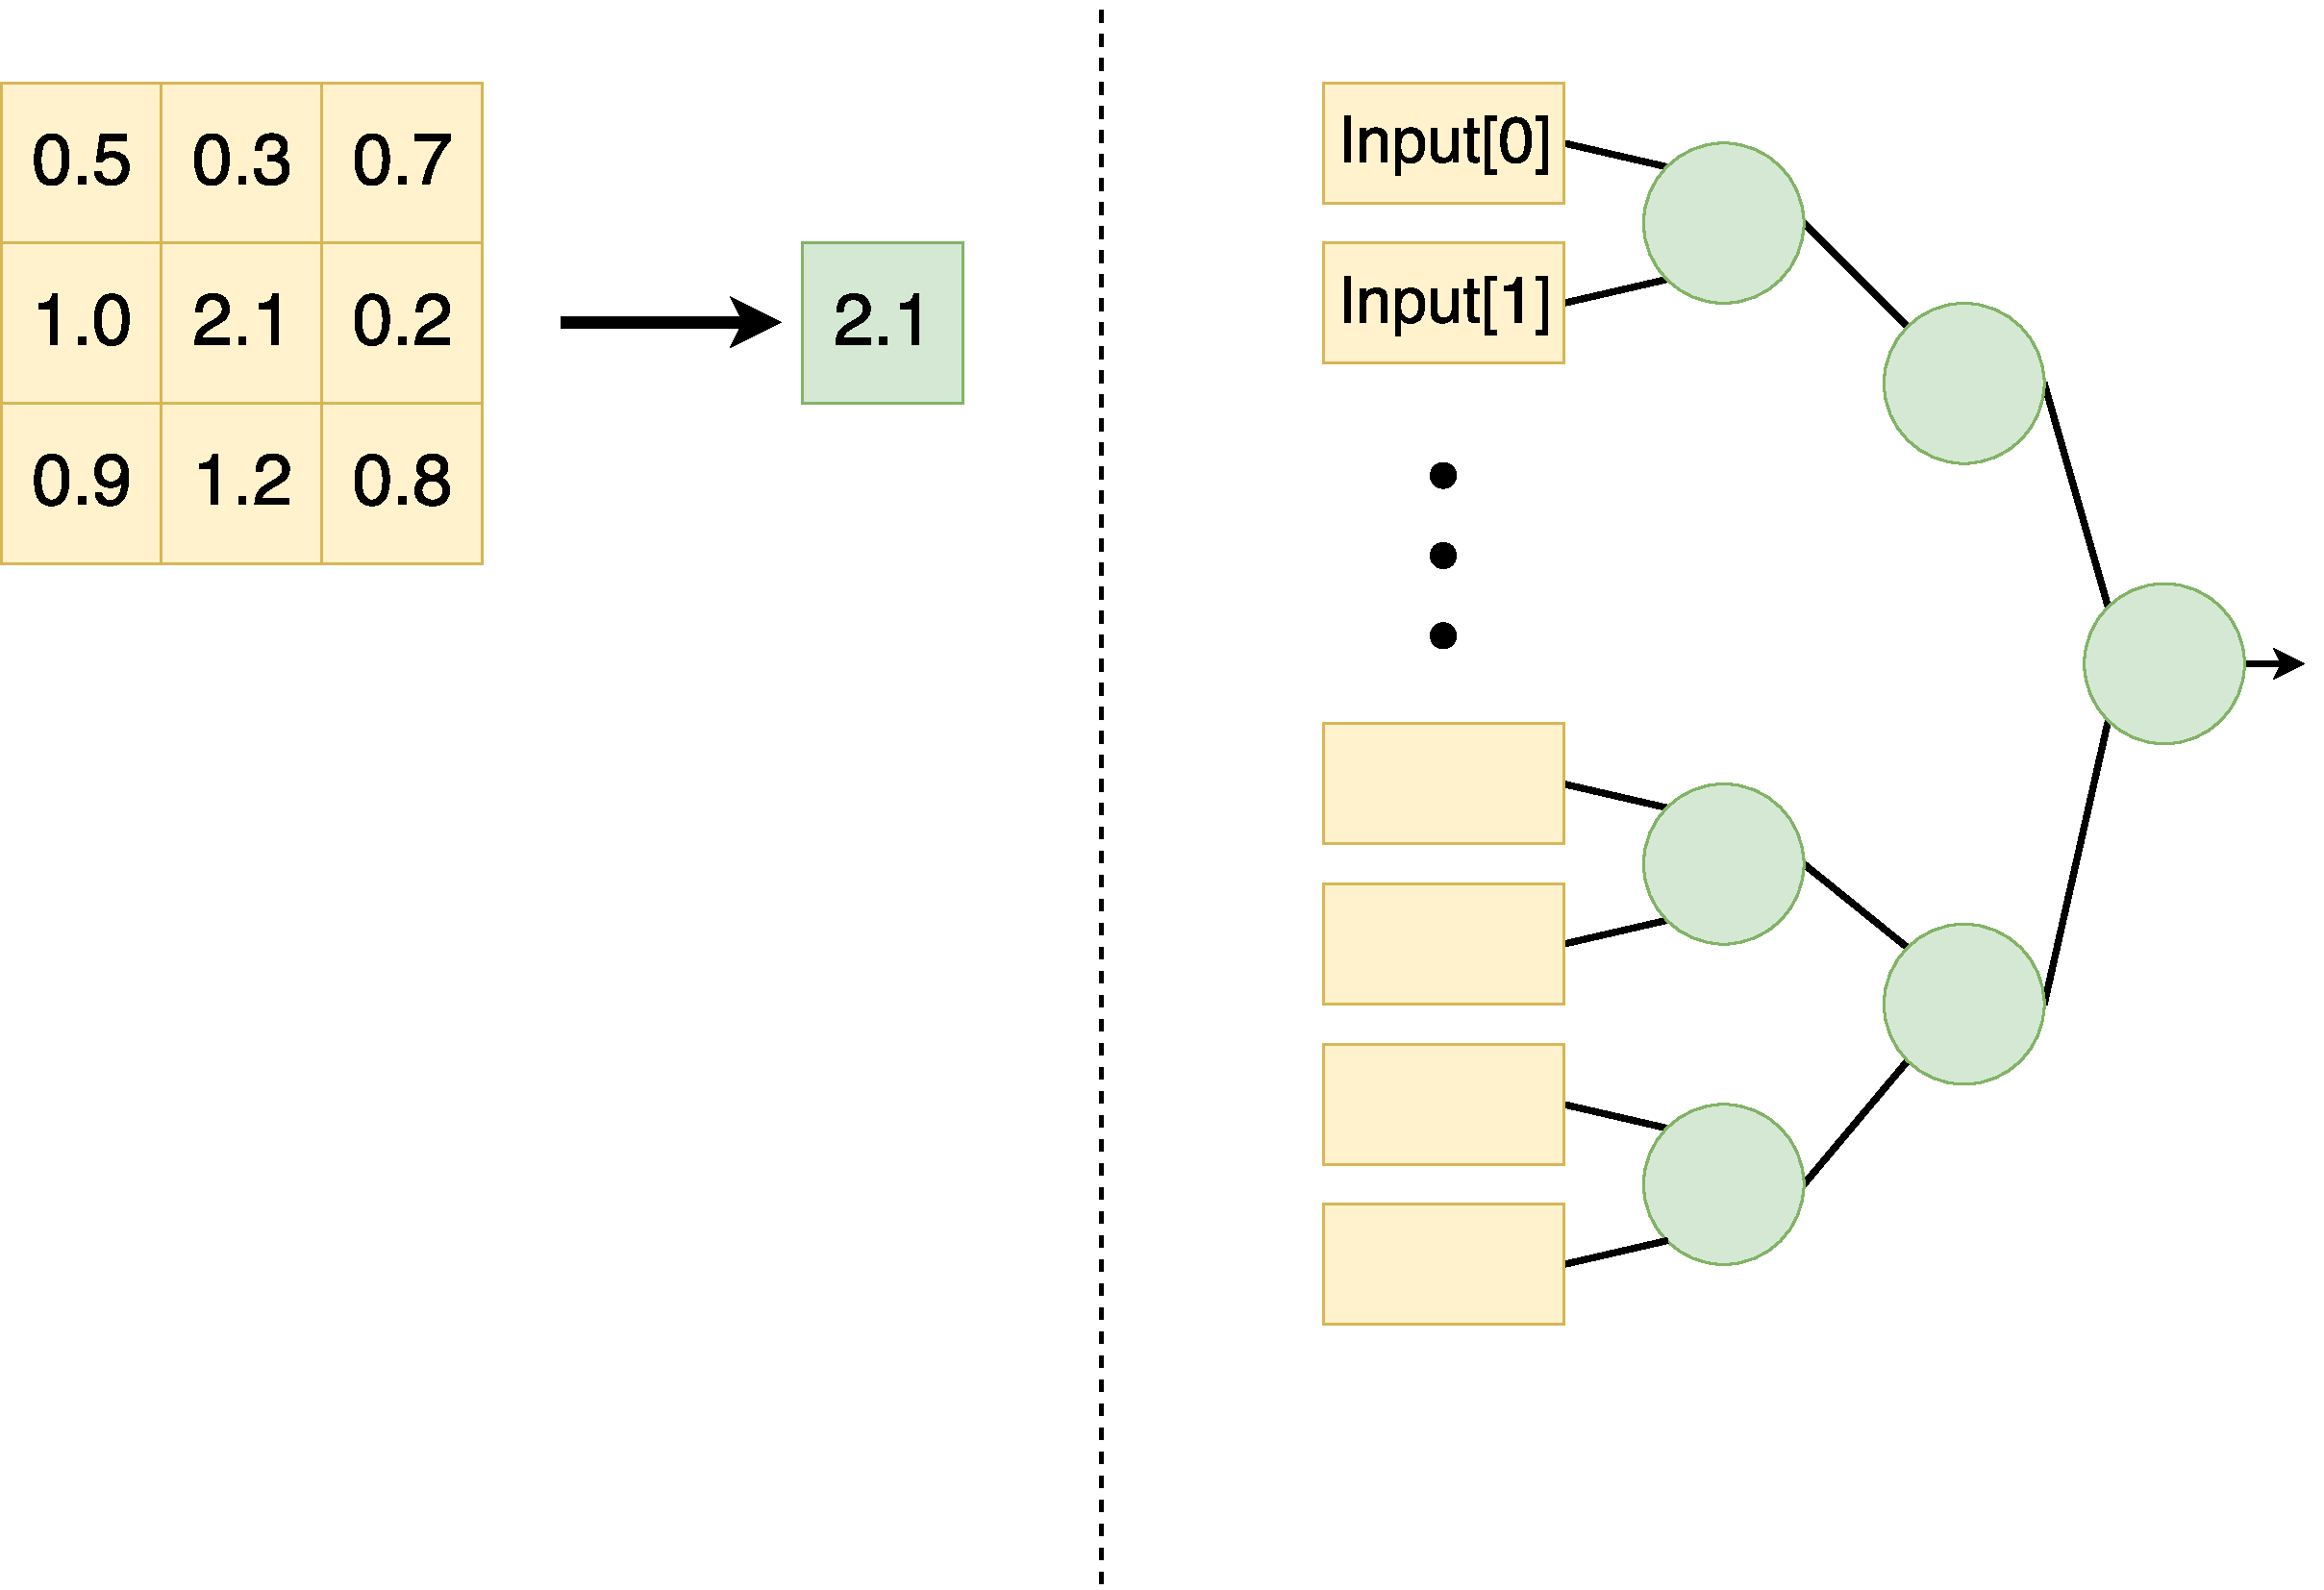
\includegraphics[width=12cm]{./chap6/fig/maxpool_pe.pdf}
  \caption{モジュールの模式図}
  \label{fig:maxpool_pe}
\end{figure}
}


\chapter{まとめと今後の課題}
{
\label{chap:conclusion}
\section{結論}
\label{sec:conclusion}
VPCMAにおいて,実行するアプリケーションと要求性能に応じて電力を最小化するパイプライン段数とボディバイアス電圧を決定する手法を検討した.トレードオフの複雑さから単純に計算することが困難であったため探索はブルートフォースで行った.4つの24bit画像処理アプリケーションを実行するシミュレーションを行い評価を行った.

パイプライン段数に着目するとVPCMAおいてはアプリケーションや要求性能によらず全段にパイプライン分割した場合がもっとも電力が小さいとわかった.この結果はVPCMA特有のものであり,ブルートフォース探索によってによって明らかとなったアーキテクチャの特徴とも言える.このように本手法ではアーキテクチャに依存せずに電力を最小化するパイプライン段数を求めることができた.

ボディバイアス制御の粒度を行単位とすることによる効果をボディバイアス制御をしない場合,制御の粒度をPE\_ARRAY全体とした場合との比較を行うことにより検討した.
ボディバイアス制御をしない場合と比べて平均約46\%の電力削減率が得られた.一方で一律制御と比べると電力削減率は平均0.80\%であった.しかし,要求性能が高くなるにつれて行単位の制御では一律制御に対して高い電力削減率を示し,その効果はアプリケーションと要求性能に依存することがわかった.

\section{今後の課題}
\label{sec:future}

本論文で検討した手法にはブルートフォース探索を採用していることはすでに述べた.そのため,パイプライン分割のパターンを制限してもパイプライン段数とボディバイアス電圧を決定するのに時間がかかっていた.このようにパイプライン段数は粗粒度に探索を行っているため本研究では想定していないパイプライン分割のパターンの方がより小さい電力を示す可能性がある.ただし,本研究で示されたように電力を最小化する段数は使用している行数の付近にあるはずであり,探索はその周辺を行えばよい.よって,本論文で提案した手法のアルゴリズムには改良の余地がある.例えば遺伝的アルゴリズムなどを代表とする進化的計算アルゴリズムを採用し得られる結果と本研究のブルートフォース探索の結果を比較することにより,この手法に適するアルゴリズムを検討する必要があると考えられる.

アプリケーション依存性があるということは,どのPEにどの演算をマッピングするかに依存するということである.本研究ではアプリケーションのマッピングは固定したままでパイプライン
段数とボディバイアス電圧を変化させて電力を見積もり最小のものを探索していた.しかし,各々のパイプライン段数,ボディバイアス電圧に対する適切な演算のマッピングは異なる可能性がある.したがって,演算のマッピングを変化させた場合の影響についても評価を行う必要があると考えられる.
}

\chapter{まとめと今後の課題}
{
\label{chap:conclusion}
\section{結論}
\label{sec:conclusion}
VPCMAにおいて、実行するアプリケーションと要求性能に応じて電力を最小化するパイプライン段数とボディバイアス電圧を決定する手法を検討した。トレードオフの複雑さから単純に計算することが困難であったため探索はブルートフォースで行った。4つの24bit画像処理アプリケーションを実行するシミュレーションを行い評価を行った。

パイプライン段数に着目するとVPCMAおいてはアプリケーションや要求性能によらず全段にパイプライン分割した場合がもっとも電力が小さいとわかった。この結果はVPCMA特有のものであり、ブルートフォース探索によってによって明らかとなったアーキテクチャの特徴とも言える。このように本手法ではアーキテクチャに依存せずに電力を最小化するパイプライン段数を求めることができた。

ボディバイアス制御の粒度を行単位とすることによる効果をボディバイアス制御をしない場合、制御の粒度をPE\_ARRAY全体とした場合との比較を行うことにより検討した。
ボディバイアス制御をしない場合と比べて平均約46\%の電力削減率が得られた。一方で一律制御と比べると電力削減率は平均0.80\%であった。しかし、要求性能が高くなるにつれて行単位の制御では一律制御に対して高い電力削減率を示し、その効果はアプリケーションと要求性能に依存することがわかった。

\section{今後の課題}
\label{sec:future}

本論文で検討した手法にはブルートフォース探索を採用していることはすでに述べた。そのため、パイプライン分割のパターンを制限してもパイプライン段数とボディバイアス電圧を決定するのに時間がかかっていた。このようにパイプライン段数は粗粒度に探索を行っているため本研究では想定していないパイプライン分割のパターンの方がより小さい電力を示す可能性がある。ただし、本研究で示されたように電力を最小化する段数は使用している行数の付近にあるはずであり、探索はその周辺を行えばよい。よって、本論文で提案した手法のアルゴリズムには改良の余地がある。例えば遺伝的アルゴリズムなどを代表とする進化的計算アルゴリズムを採用し得られる結果と本研究のブルートフォース探索の結果を比較することにより、この手法に適するアルゴリズムを検討する必要があると考えられる。

アプリケーション依存性があるということは、どのPEにどの演算をマッピングするかに依存するということである。本研究ではアプリケーションのマッピングは固定したままでパイプライン
段数とボディバイアス電圧を変化させて電力を見積もり最小のものを探索していた。しかし、各々のパイプライン段数、ボディバイアス電圧に対する適切な演算のマッピングは異なる可能性がある。したがって、演算のマッピングを変化させた場合の影響についても評価を行う必要があると考えられる。
}

\chapter{謝辞}
{
本研究に取り組むにあたりご指導ご鞭撻を賜りました天野英晴教授,に深く感謝いたします.
主査をしていただくとともにVivadoの使い方、アクセラレータ実装での助言を頂いた武者千嵯氏、副査として
論文の基本的な書き方を教授してくださった安戸僚汰氏にも深く感謝いたします。

}

%-end body-----------------------------------------%


%-reference----------------------------------------%
\bibliographystyle{junsrt}
%\nocites{*}
\bibliography{bibdata}
%-end reference------------------------------------%
\end{document}
